\documentclass[conference]{IEEEtran}
\IEEEoverridecommandlockouts
% The preceding line is only needed to identify funding in the first footnote. If that is unneeded, please comment it out.
\usepackage{cite}
\usepackage{amsmath,amssymb,amsfonts}
\usepackage{algorithmic}
\usepackage{graphicx}
\usepackage{textcomp}
\usepackage{xcolor}
\usepackage{url}
\usepackage{tabularx}
\usepackage{tabulary}
\usepackage{svg}
\usepackage[scaled=0.8]{FiraMono}

\def\BibTeX{{\rm B\kern-.05em{\sc i\kern-.025em b}\kern-.08em
    T\kern-.1667em\lower.7ex\hbox{E}\kern-.125emX}}
\begin{document}

\title{\textsc{Ferret Miner}: A Process Mining Case
Study${}^\dagger$\thanks{${}^\dagger$~Github: \texttt{https://github.com/Martin-Chivo/CMPE255-Team8}; Google Drive: \texttt{shorturl.at/cgFIP}}}

\author{\IEEEauthorblockN{Martin Alvarez-Lopez${}^1$\thanks{${}^1$~MS Candidate in Software Engineering, San José State University}}
% \IEEEauthorblockA{San José State University}
\and
\IEEEauthorblockN{Carlos Hernandez${}^2$\thanks{${}^2$ MS Candidate in Computer Engineering, San José State University}}
% \IEEEauthorblockA{San José State University}
\and
\IEEEauthorblockN{Hardy Leung${}^3$\thanks{${}^3$ MS Candidate in Artificial Intelligence, San José State University}}
% \IEEEauthorblockA{San José State University}
\and
\IEEEauthorblockN{Divyam Sobti${}^3$}
% \IEEEauthorblockA{San José State University}
}

\maketitle

\begin{abstract}
This project is a process mining case study designed to
identify patterns and
delays that obstruct the efficient flow of process
activities. Specifically, our
objective is to analyze event data logs from
the travel reimbursement process at Eindhoven University of Technology
(\textsc{tu/e}), identify bottlenecks in the process, and
seek improvement to its efficiency.
We prepare and filter the event data, and then generate simplified and
representative process models to locate
the most time-consuming and impactful critical tasks.
Our analysis suggests that
improvement in the supervisor approval and payment handling activities 
could significantly
reduce the time processing the travel reimbursement.
\end{abstract}

\begin{IEEEkeywords}
process mining, data, conformance, event logs
\end{IEEEkeywords}

\section{Introduction}
\label{section-intro}


Nowadays, most organizations use information systems to support
the execution of their business processes, generating significant
amounts of data.
Mainstream information systems, such as Enterprise Resource
Planning (\textsc{erp}), Work on Management Systems (\textsc{wms}), and Customer
Relationship Management (\textsc{crm}), have become vital tools behind the
operation of almost 
any company process\cite{Tuto2022}. All of these platforms
offer rich event logging capabilities, in which
an event log is
basically a record of an activity performed with a timestamp embedded
\cite{Proc2022}.

There are plenty of oppportunities, through
proper supervision of business behavior, to identify and adjust
tasks that are generating problems for the business processes
\cite{LeAl1994}.
One important technique towards such goal is process mining, a
specialized data analysis technique that reveals core business behavior
indicated by activity logs.
Process mining would start with these event logs, extracting important
information including the chronology of the activities
 and their execution time registered in each log. Representative models
would be built, or discovered automatically,
and then be used to detect errors and deficiencies in the process,
and to provide insight and suggestions for process enhancement.
Process mining is most closely related to data mining 
amongst business intelligence disciplines. However,
while data mining focuses on finding relationships among data,
process mining also looks at data from a systematic
perspective.

\subsection{Problem Description}

In our process mining case study, we investigated
a dataset with
real-life event log data from the travel reimbursement process at
Eindhoven University of Technology (\textsc{tu/e}). Through analyzing the event
logs and mining the business process underlying the events, we seek to
identify and suggest remedies to address deficiencies in the reimbursement
process.
The event logs provide a detailed record of the travel reimbursement process,
including important attributes such as identification, resources,
timestamp, permits, payment and budgeting information, and event labels.
Students or staff would submit their reimbursement applications,
provide suppport documentation (especially
for international travels), wait for
reimbursement decision and subsequent payment, and possibly deal with
rejection and resubmission.
Collectively, these information provided a substantial amount of detail
into the reimbursement workflow. 
The data was obtained from 
the annual \textsc{bpi} Challenge as part of
the 2020 International Conference on Process Mining \cite{BPI2020}.

Our approach to process mining is based on the work by
Wil van der Aalst in his seminal paper titled simply
``Process Mining'' \cite{van2012},
while offered detailed process mining guidelines.
A process mining implementation generally
covers three main issues: (1) discovery, (2) conformance,
and (3) enhancement.
Our project focuses on discovery since it is the area
that requires the most effort and it is the most deterministic for the
success of the analysis. We will also take a cursory
look at conformance as both an aide to discovery and a motivation for
future work.

\subsection{Motivation}

Publications on practical application of process mining are scarce,
and our research paper aims to add support to this area. Our goal is
to demonstrate the practicality of process mining and analysis
in practice, in application to the real-life travel reimbursement problem
as detailed earlier.

Furthermore, we are very interested in the evaluation and application
of an emerging process mining approach based on
\textsc{pm4py}, a Python process mining library
developed by Berti et al.~\cite{BeZe2019}.
According to the authors,
\textsc{pm4py} is a modern, open-source, and extensible platform developed
specifically for the data science community. Prior to the turn of the
millenium,
there were hardly any tooling for process mining, but
since then a slew of software tools, both open-source
(\textsc{prom} and \textsc{apromore}) and commercial
(\textsc{disco}, \textsc{celonis}, and \textsc{processgold}),
have been developed for process mining.
Yet, many were proprietary, hard to extend,
or hidden behind graphical user interfaces.
The conservative mindset of process mining
tooling contrasted greatly with the modern philosophy of data science
R\&D,
which put significant emphasis on openness and extensibility.
\textsc{pm4py} was developed to bridge the gap
and bring process mining to mainstream data science
capabilities such as
\textsc{pandas}, \textsc{numpy}, \textsc{scikit-learn}.
We whole-heartedly
agree with the assessment of the authors, and look forward to opportunities
that the \textsc{pm4py} approach brought forth, including
the adoption of modern and rapidly evolving machine learning
techniques to process mining.


\subsection{Approach Summary}

This document is structured as follows: Sections \ref{section-intro} and
\ref{section-survey}
offer an introduction to process mining and a literature survey.
Sections \ref{section-technical}, \ref{section-methodology} and
\ref{section-models} describe the technical details of our methodology, as
well as the results of our investigation. We will end the paper with
future work in Section \ref{section-future} and conclusion in
\ref{section-conclusion}.

\section{Survey}
\label{section-survey}

In this section, we shall offer a very brief review of the literature
on process mining, focusing on the development of techniques
and algorithms from a control-flow discovery perspective, as well as
 its applications.

\subsection{Process Mining}

Van der Aalst et al.~described the discipline of process mining as positioned
somewhere between data mining and process modeling
\cite{van2004}. Process mining interacts with the rest of the software
ecosystem
mainly through the language of event logs (see Figure \ref{fig-outline}),
and the objective is to provides useful information
with implication on the business processes, organizations, and people involved.

\begin{figure}[htbp]
\centerline{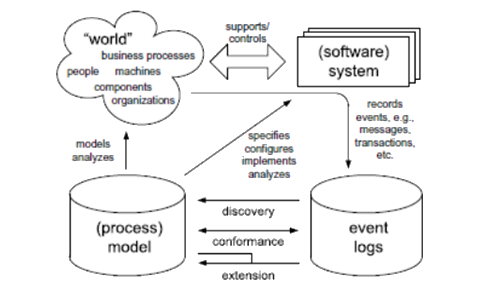
\includegraphics[width=0.45\textwidth]{images/image2a.png}}
\caption{General outline of process mining approach.}
\label{fig-outline}
\end{figure}

Although information system databases capture important business data
in the form of event logs, they do not
usually provide understanding of the data in a structural or systematic manner.
Traditionally, process analysts must search for and
retrieve the information directly from the system, and perform manual
analysis to accomplish their specific objectives.
To put it another way, event logs only possess
the right information, but not the right insight.
Whether or not a process mining implementation is successful or applicable
thus largely hinges on what it can do with the event logs
\cite{van2012}. As such, process mining approach must
embrace three main actions (Figure \ref{fig-layout}):

\begin{itemize}
\item \textit{Discovery} --
create robust and representative process models through
 analyzing event logs.

\item \textit{Conformance} -- verify and compare newly created
models against either the event logs or other predefined models
to gain knowledge.

\item \textit{Enhancement} -- turn the analysis 
into insights and suggestions to overcome previously
detected problems.
\end{itemize}

\begin{figure}[htbp]
\centerline{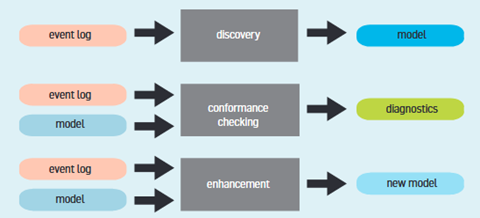
\includegraphics[width=0.4\textwidth]{images/image1.png}}
\caption{General outline of process mining approach.}
\label{fig-layout}
\end{figure}

\subsection{Process Models}

Many distinct data analysis approaches have been developed to discover
processes from event logs. However, \textsc{petri net}s\footnote{\textsc{petri net}s are also
equivalent to \textsc{bpmn} models and process trees.} have become a
widely adopted technique over other methods \cite{Cook1998} due to their
intuitiveness, mathematical soundness, and ease of analysis.
Another approach utilizes Unified
Modeling Language (\textsc{uml}) diagrams \cite{Sait2019}.
In 2004, van der Wilst et al.~described the 
a break-through algorithm in process mining
called \textsc{alpha miner}\cite{van2004} which
is capable of distilling event data logs into
work-flow diagrams, which can then be translated to \textsc{petri net}s.
The success of \textsc{alpha miner} has inspired many follow-up
publications,
including a popular model
called \textsc{heuristics miner} \cite{Weij2006}.
One main characteristic of this
algorithm is its high level of configurability and flexibility.
In order to deal with the
massive number of events that actual information systems generate,
Burattin et al.~\cite{Bura2014} developed another extension to
\textsc{heuristics miner} based on
lossy counting, as well as a sliding window that effectively analyzes
streams of real datasets.

\subsection{Applications}

Most process mining publications are dedicated mainly to the enhancement
of novel methodologies and algorithms with significant emphasis on the
control-flow discovery area \cite{van2004}. However, the public services area
has been fruitful ground
for process mining deployment research. For instance, a
genetic miner approach was tested by de Madeiros et al.~\cite{deMe2007}
in Dutch municipalities. Additionally, van del Aalst et al.~\cite{RoDJ2009}
applied an analysis of organizations in another municipality process.
Rozinat et al.~\cite{RoMa2009} evaluated process models in two different case
studies on the public sector.

Implementation of process mining approaches has also been done in
the private domain. Distinct discovery approaches were
deployed by Goedertier et al.~\cite{GoDW2011} in the field of
telecommunication. Mans
et al.~\cite{MaSc2008} and Rebuge et al.~\cite{ReBu2012} both
evaluated process mining methods
to resolve the tracking of patients within the healthcare industry.

\section{Technical Approach}
\label{section-technical}

We shall now briefly describe our approach to finding
where the process bottlenecks are. We would start with a thorough analysis and
cleaning of the event logs, and then
build models that best capture the behavior of the
process, making the proper tradeoff
between robustness (whether the model captures the intent of the process),
and coverage (what fraction of the traces are modeled).
 Then, we will use the
chosen models to answer the questions we hade in mind.

We shall note that process mining is a relatively new and unfamiliar
technique, and
as such we spent a disproportional amount of time ramping up the project.
While we completely believe in the full potential of \textsc{pm4py} due to
its focus on algorithmic discovery and availability
on Python, it is
essentially still an academic software in its nascent stage, and 
hence suffers from many issues such as software instability,
limitation in visualization and presentation, scanty documentation,
and immaturity in API design.  There is still plenty of room for
improvement.

\section{Methodology}
\label{section-methodology}

In this section we will discuss about the data, 
how we preprocessed it, what model we used, and how
we reached the results and the insight we obtained.

\subsection{Description of the Dataset}

After a thorough review of what our tasks entail, we decided to focus
exclusively on the domestic and international travel event logs in order
to identify the process bottlenecks.  Both event logs
were provided to us in \textsc{xes} format,
an \textsc{xml}-based standard for event logs \cite{XES2021}, which can
be easily parsed using \textsc{pm4py}.
The events are organized as a two-level hierarchy as follows:
An event log is made of a list of cases
(also known as traces in research
terminology), and each case is made of a list of timestamped events. Cases and
events are both extensible constructs to allow for maximum flexibility in
event modeling.

The event logs provide a detailed record of the travel reimbursement process,
including important attributes such as identification, resources,
timestamp, permits, payment and budgeting information, and event labels.
Students or staff would submit their reimbursement application,
provide suppport documentation (if traveling internationally), wait for
approval and payment, and resubmit a corrected request if rejected.

The logs that were imported into Python via 
\textsc{pm4py} were converted into
dataframes, a key construct of
\textsc{pandas}, the popular Python Data Analysis Library. However, as
dataframes are not hierarchical, \textsc{pm4py} flattened the logs so that 
the enclosing case and the case attributes
became attributes of the event. If
there were $A_C$ attributes associated with a
case, and $A_E$ event attributes in the
\textsc{xes} specification, after \textsc{pm4py} import, we would obtain a
\textsc{pandas} dataframe 
with $N$ events, each with a total of $A_C + A_E$ attributes.

In our project,
the domestic process log is organized differently than
the international process log.  For domestic trips, employees would first
complete the trip and then ask for reimbursement. On the other hand,
the policy for international trips mandates that
employees first obtain travel permits from the supervisors prior to
commencing their trips.

As a result, the reimbursement process for international travel is
far more complex, and the formal specification that describes
international cases also contain more fields.
Specifically, while domestic cases only have 5 attributes
each, international cases have 13 additional attributes, on top of
the 5 attributes shared with domestic cases
(\texttt{id}, \texttt{concept:name}, \texttt{BudgetNumber},
\texttt{DeclarationNumber}, \texttt{Amount}), for a total of 18 attributes.
Regardless of the type of trips, however,
the event in the \textsc{xes} hierarchy has the same 5 attributes
(\texttt{id}, \texttt{org:resource}, \texttt{concept:name},
\texttt{time:timestamp}, and \texttt{org:role}).
After flattening, \textsc{pm4py} returned a
domestic dataframe with $56437$ events and $10~(=5+5$) attributes, and
an international dataframe with $72151$ events and $23~(=18+5$) attributes.
To avoid namespace collision, all case attributes were prefixed with
\texttt{case:} by \textsc{pm4py} (for example, the \texttt{id} field of a case
became \texttt{case:id}). Please refer to Table
\ref{table-event} for a complete list of all attributes:

\begin{table}[htbp]
\caption{XES Attributes for Events, and Domestic and Int'l Cases}
\vspace{-1em}
\begin{center}
\begin{verbatim}
  XES Event Attributes (5 Total)
    ---------------------------------------------------------
    id, org:resource, concept:name, time:timestamp, org:role
    ---------------------------------------------------------

  XES Domestic Case Attributes (5 Total)
    ---------------------------------------------------------
    id, concept:name, BudgetNumber, DeclarationNumber, Amount
    ---------------------------------------------------------

  XES International Cases (18 fields)
    ---------------------------------------------------------
    Permit travel permit number, DeclarationNumber, Amount,
    RequestedAmount, Permit TaskNumber, Permit BudgetNumber,
    OriginalAmount, Permit ProjectNumber, concept:name,
    Permit OrganizationalEntity, travel permit number,
    Permit RequestedBudget, id, Permit ID, Permit id,
    BudgetNumber, Permit ActivityNumber, AdjustedAmount        
    ---------------------------------------------------------
\end{verbatim}
\end{center}
\vspace{-1em}
\label{table-event}
\end{table}


% Unique noise coming from outside processes, difficult to identify.
% Cannot use statistics to view outliers. There were no null or missing values.

Prior to process mining, we performed a thorough cleaning of the
domestic and international dataframes to ensure we have
the best possible starting
point for analysis. There were three categories of modification we applied
to the datasets:

\subsection{Data Preprocessing I -- Missing Values}

While we did not find any missing value per se (as far
as \textsc{pandas} is concerned), we did find columns with string values
\textsc{unknown} or \textsc{missing}. We
carefully evaluated what to do with these attributes on a case-by-case
basis. For example, we could drop the column (attribute), drop the row
(event), fill the missing values, or simply ignore the column.

In the case of international reimbursement, we decided that we should
drop events without a permit number. The permit number is actually a
concept of the case, and hence we were removing traces without permit
number in their entirety. This would turn out to be the most significant
modification to our international dataset.
% , reducing the number of events
% from 72151 to 45045, or 38\%.
We believe this is justified, because a trip
without any associated permit violated the very fundamental assumption
about the international reimbursement process, that there is a permit
associated with the trip. Note that the decision to drop these entries was
not ``lossy'', because international reimbursement request without a permit
number \textit{should} have been rejected and not entered into the system
in the first place.

\subsection{Data Preprocessing II -- Duplicated Attributes}

Perhaps due to prior inconsistency between
versions of the enterprise software, there are fields that are similar
or duplicate of each other. For example, \texttt{Permit ID}, \texttt{Permit id},
and \texttt{Permit travel permit number} are one and the same.
Moreover, it is quite likely that exactly one of the three fields were
filled, while the others are missing (or reported as
\textsc{missing}. We combined these similar fields into one, picking out
the value from the non-missing column, and dropped the duplicates. Note that 
we performed this duplicate analysis prior to future treatment of missing
values.

As a result of these cleaning procedures, the size of the
the international dataframe was reduced from 72151 to 43707 (a 60\% drop),
with the
missing permit accounting for 95\% of such reduction. The number of
columns was reduced from 23 to 19, since we dropped
several permit-related columns that are duplicates.
Similarly, the domestic dataframe was also modified to a much small extent.
The number of events was reduced from 55087, a mere 2\% drop, and the
number of columns stayed the same.

\subsection{Data Preprocessing III -- Infrequent Events}

Process models that can explain all possible event traces could be
arbitrarily complex. For example, obviously we would expect reimbursement to
be paid out only after the request was approved. But what if there is
a trace with a missing approval due to erroneous logging? A process model
built to handle 100\% of traces must handle a flow with
payment before request, however bizzare such trace is.
Not only would the model be more complex and unwieldy,
it would also be incorrect and fail our objective.

A naive approach would be to remove events that are uncommon, but doing so may
not be sufficient. Consider the previous example;
while \textsc{request approved} that happened after \textsc{payment handled}
might be a rare sequence, neither of these events were rare.

In \textsc{pm4py} terminology, the variants of an event log is the
union of all possible sequences of event execution (ignoring all but the
event labels). For example, there were
68 variants in the domestic log, and 464 variants in the international log.
In fact, the above example
points to the need to remove traces that are uncommon. Clearly, it could
be beneficial to have the choice to build the process model based on
only the most popular traces. Indeed, this was an important part of our
methodology and we shall take a closer look in the next section.

\section{Models and Results}
\label{section-models}


With the event logs well understood and properly prepared, we are now
ready to build the actual process model.

\subsection{Choice of Model}

We must first answer the
question of what formal model to use. Our choices include \textsc{bpmn}\footnote{\textsc{bpmn} stands for Business Process Model Notation}  model,
process tree, \textsc{petri net}, and Directly-Follows Graph (\textsc{dfg}). The
first three are mathematically equivalent and inter-changeable. On the other
hand, \textsc{dfg} shows a different view of \textsc{bpmn} graph constructed by aggregrating all possible link
between any pair of events that follows each other.

There are pros and cons in choosing \textsc{petri net} vs \textsc{dfg}. \textsc{dfg}s can be constructed
directly from the event logs, and are simple to understand. \textsc{petri net}s (as well
as the equivalents) can only be generated heuristically, for example, 
through inductive or heuristics miners (which \textsc{pm4py} supports).
The difference mainly lies on how concurrency is handled. For example,
say there are two activities $X$ and $Y$ that are sandwiched between
$A$ and $B$. In other words, the following are both legitimate sequence
of executions:

\vspace{0.5em}
$\phantom{xxxxx}A \rightarrow X \rightarrow Y \rightarrow B$

$\phantom{xxxxx}A \rightarrow Y \rightarrow X \rightarrow B$
\vspace{0.5em}


While both \textsc{alpha miner} and \textsc{inductive miner} would correctly deduct
(probabilistically) that $X$ and $Y$ have no inter-dependency but are
instead concurrent events, \textsc{dfg} would not be able to discern that, because
all it saw was $Y$ directly follows $X$ in the first example, and
$X$ directly follows $Y$ in the second. Thus, concurrency would
show up in \textsc{dfg}s as tight loops between two activities, yet there is no
way to prove that tight loops imply concurrency. If indeed \textsc{dfg}s
become too complicated, they will confuse rather than aide reasoning.

For our purpose, however, we still believe 
is the preferred approach as the statistics on the edges of a \textsc{dfg} can be
made readily available, and more easily reasoned with. We just need to make
sure we have a model that is not too complicated.
This speaks to the importance of limiting the model size, which we shall
discuss next.

\subsection{Choice of Model Size}

How many top variants do we use to build the model?
We did experiment with different values of $k$, where $k$ is the number of
top variants to be used to build the \textsc{dfg}. We
evaluated many factors, though more qualitatively than otherwise,
and came to the conclusion
that we would achieve the best balance between coverage and robustness if
we keep approximately 15 to 25\% of the top variants, depending on data
(higher for domestic, and lower for international). Figures~\ref{fig-domestic}
and \ref{fig-international} shows the \textsc{dfg} models we picked for
domestic and international reimbursement respectively. In each figure,
the \textsc{dfg} to the left is annotated with the number of directly following
edges, and the \textsc{dfg} to the right is annotated with the mean duration between
the two events. Both models captured the vast majority of the important
interactions very well and were reasonably easy to comprehend.

\begin{figure*}[htbp]
\centerline{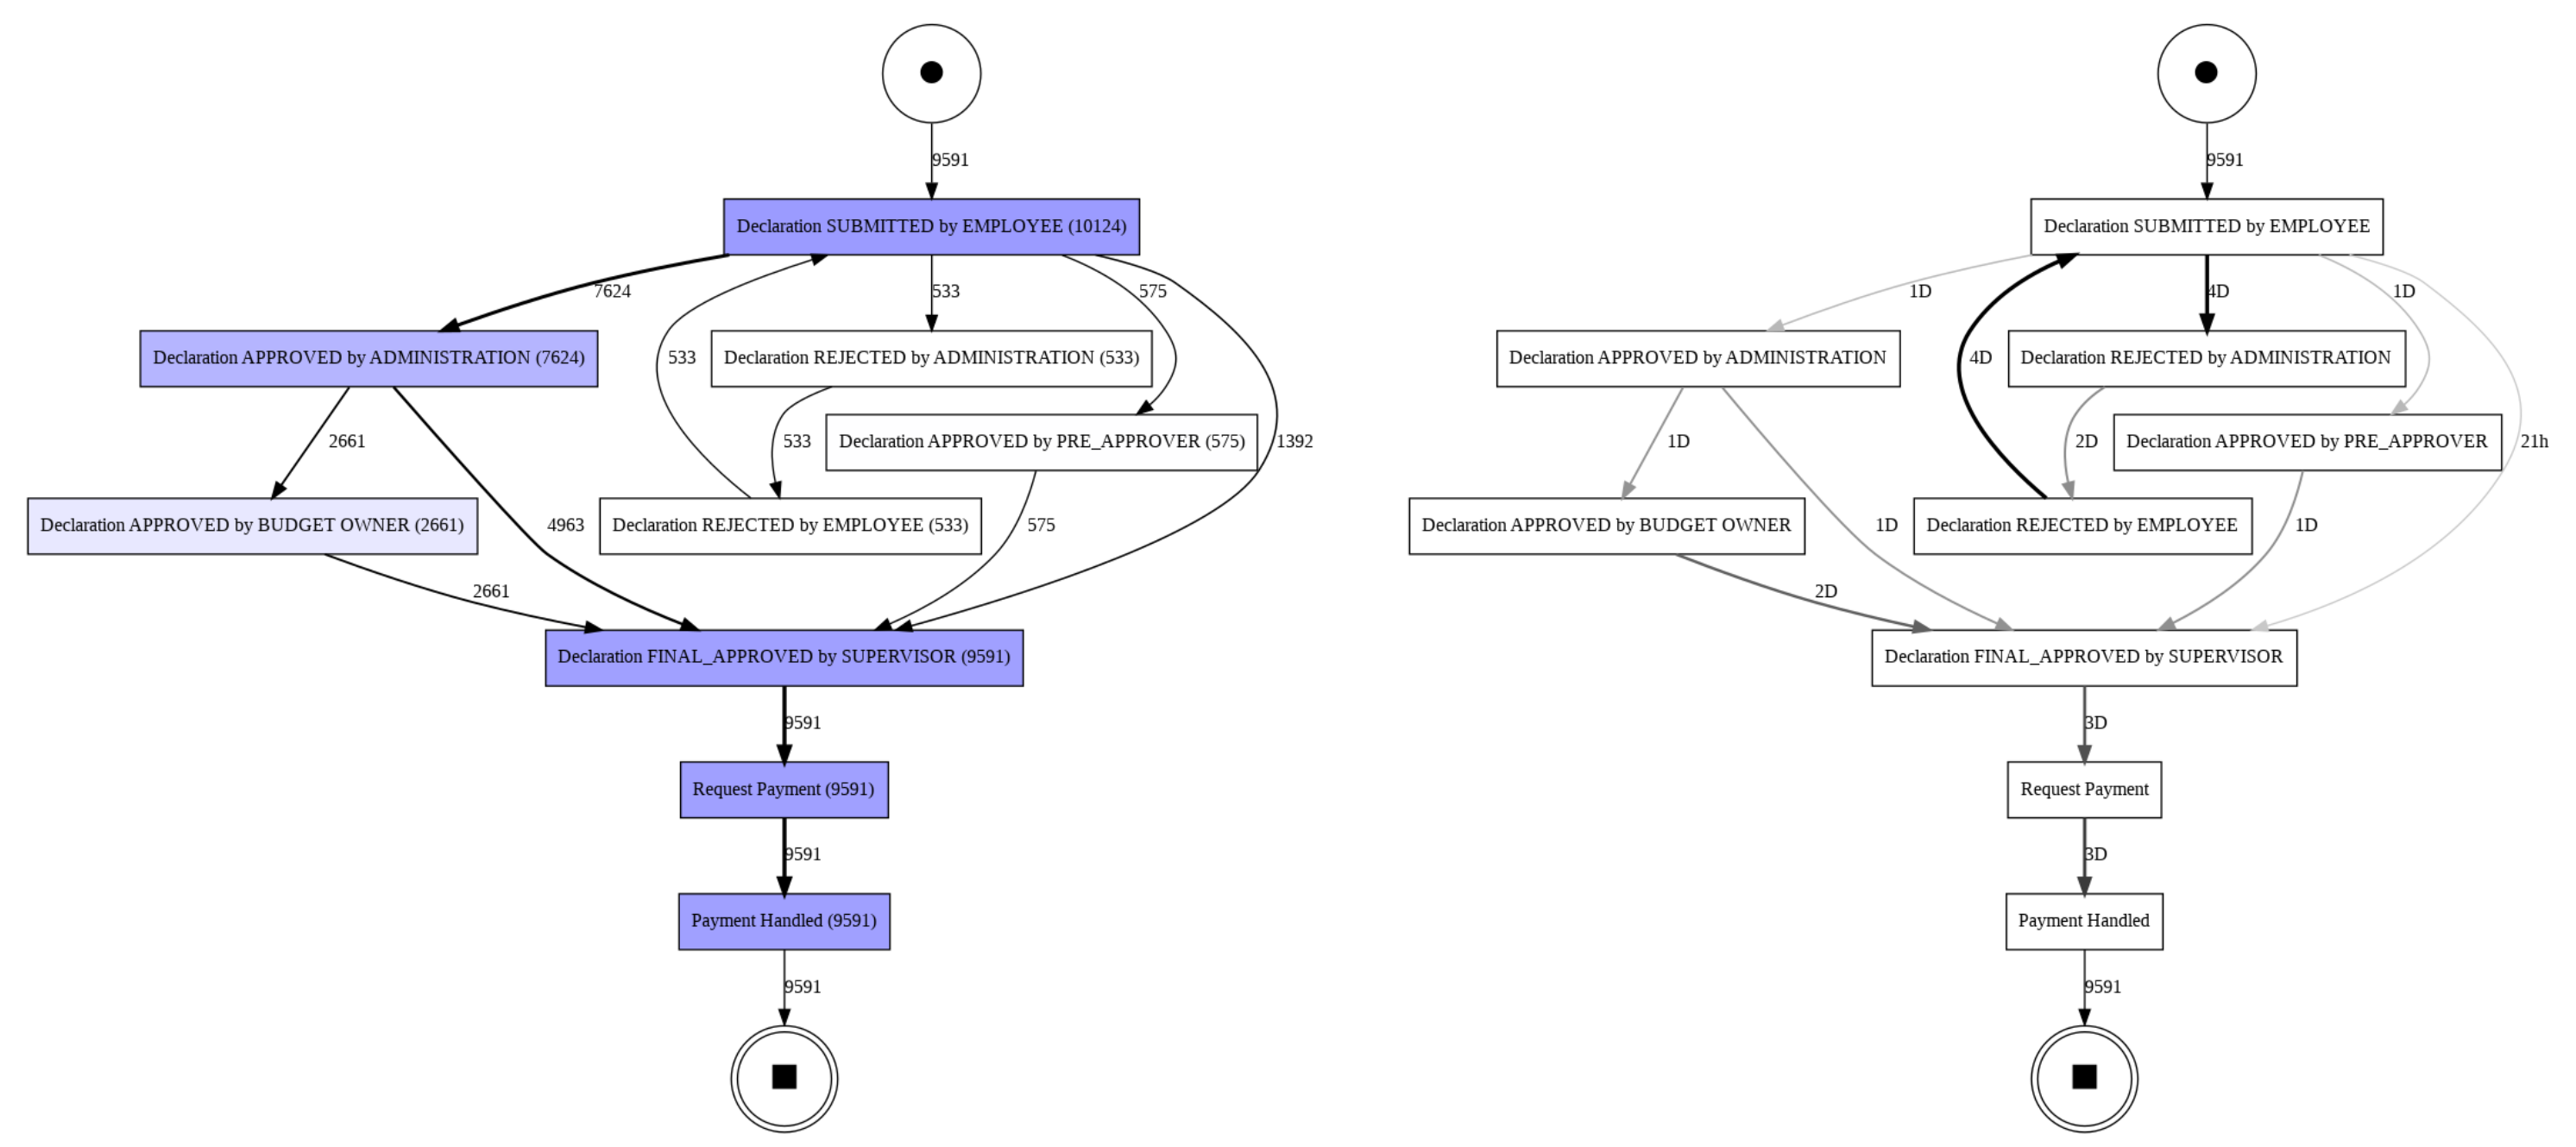
\includegraphics[width=0.60\textwidth]{images/domestic.png}}
\caption{\textsc{dfg} Model for Domestic Reimbursement.}
\label{fig-domestic}
\end{figure*}
\vspace{-1em}

\begin{figure*}[htbp]
\centerline{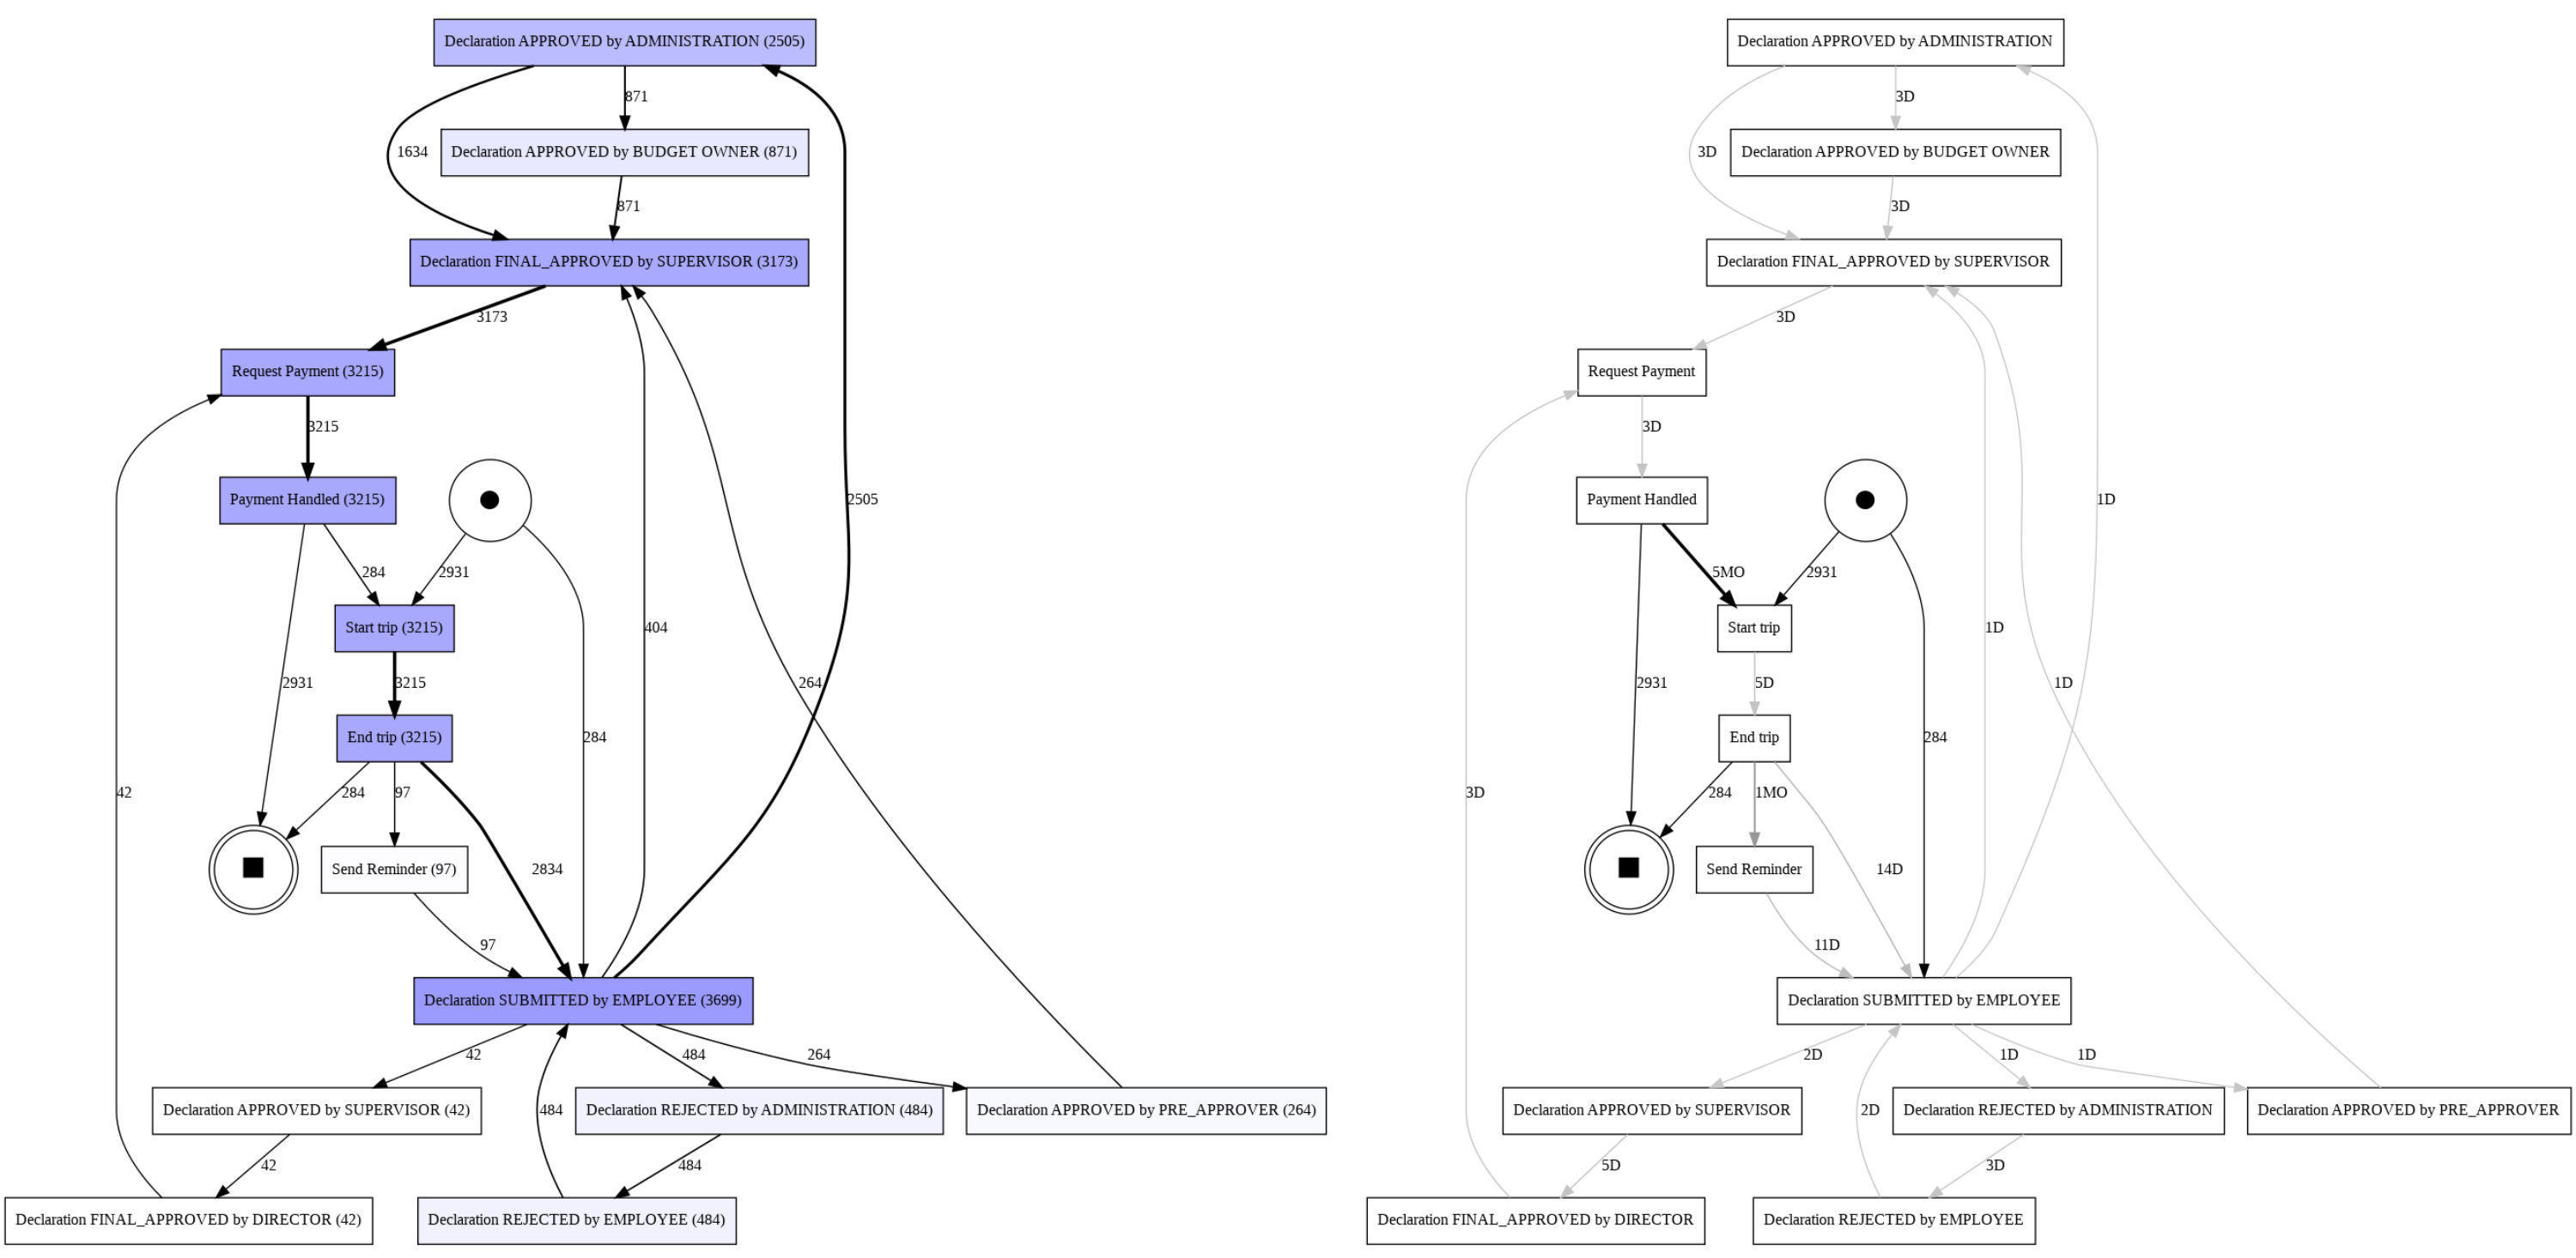
\includegraphics[width=0.60\textwidth]{images/international.png}}
\caption{\textsc{dfg} Model for International Reimbursement.}
\label{fig-international}
\end{figure*}
\vspace{-1em}


\subsection{Results}

Now that we have a robust process model built on reasonably clean data,
we can now answer the question: 
Where are the bottlenecks in the process of a travel declaration?

The biggest bottleneck is the supervisor activities for both international
and domestic declarations.  For the supervisor to do the final approval and
request payment, it takes an average of 4 to 5 days.
To find such bottleneck, we would identify that
links with both high frequency \textit{and} long duration. Since the models
are simple enough, we were able to visually inspect the models and identify
such link. We did add code to work around \textsc{pm4py} and
automatically identify such links.

On the other hand, if we
were to identify one activity, \textsc{Payment Handled}
is the biggest bottleneck. That said,
it might be outside of the organization’s control and may be more of a
financial institution issue.

% Note that \textsc{pm4py} does not allow us to customize the performance
% graph output,
% instead, it rounds up the time to days instead of
% leaving it in an hour format.
% Also, \textsc{pm4py} does not have a method of superimposing the
% frequency and performance.

\section{Future Work}
\label{section-future}

Now we shall look into two potential area of work in the future --
conformance analysis and machine learning.

\subsection{Conformance Analysis}

Once we have developed a process model either extracted through process
discovery, or built on some reference guidelines. It would be
interesting to investigate further into conformance checking to see how
well the data fits the model, while in turn would help us evaluate and
improve on the model.

This can be done with a method called token-based replay (\textsc{tbr}) on the
\textsc{petri net} converted from the process model. For each trace, we would try
to see if it can be simulated on the \textsc{petri net} which can be done
precisely in a mathematically sound
way. We define the total fitness
simply as the percentage of traces that fit the model. Other techniques
we can apply are 
alignment analysis and behavior analysis, though
they both come at the expense of higher runtime complexity.
Together these techniques can be used to better identify the hows and whys of
non-conformance, and to build better models.
In conformance analysis,
getting to 100\% total fitness is not a desired goal, as explained earlier.
Instead, what we seek is a tradeoff. On the one hand, you want the model
to be robust enough to elegantly explain the process. On the other hand,
we do not want to over-build a model so complex that it is impossible to
reason about.

Let's use our specific problem as an example. We
ran an experiment to examine the tradeoff between fitness and model
complexity. We built the model multiple times with \textsc{inductive miner},
each time on a different value of $k$, where $k$ is the number of top
variants we
used to build the model, and we recorded the total fitness via conformance
check, as well as an estimate the complexity of the model computed using
custom Python code.
In Figure~\ref{fig-tradeoff}, the
red line is the total fitness, and the blue line is the size of the
model. We see that, as we include more top variants, the model gets more
complex, but the fitness also improves. If we would include only the top
3 variants, we can already explain 90\% of the traces. But if we blindly
crank up the knob to 
18 variants, the model would now account for 99\% of the traces, but the
it is 5 times bigger, and much harder to understand.

\begin{figure}[htbp]
\centerline{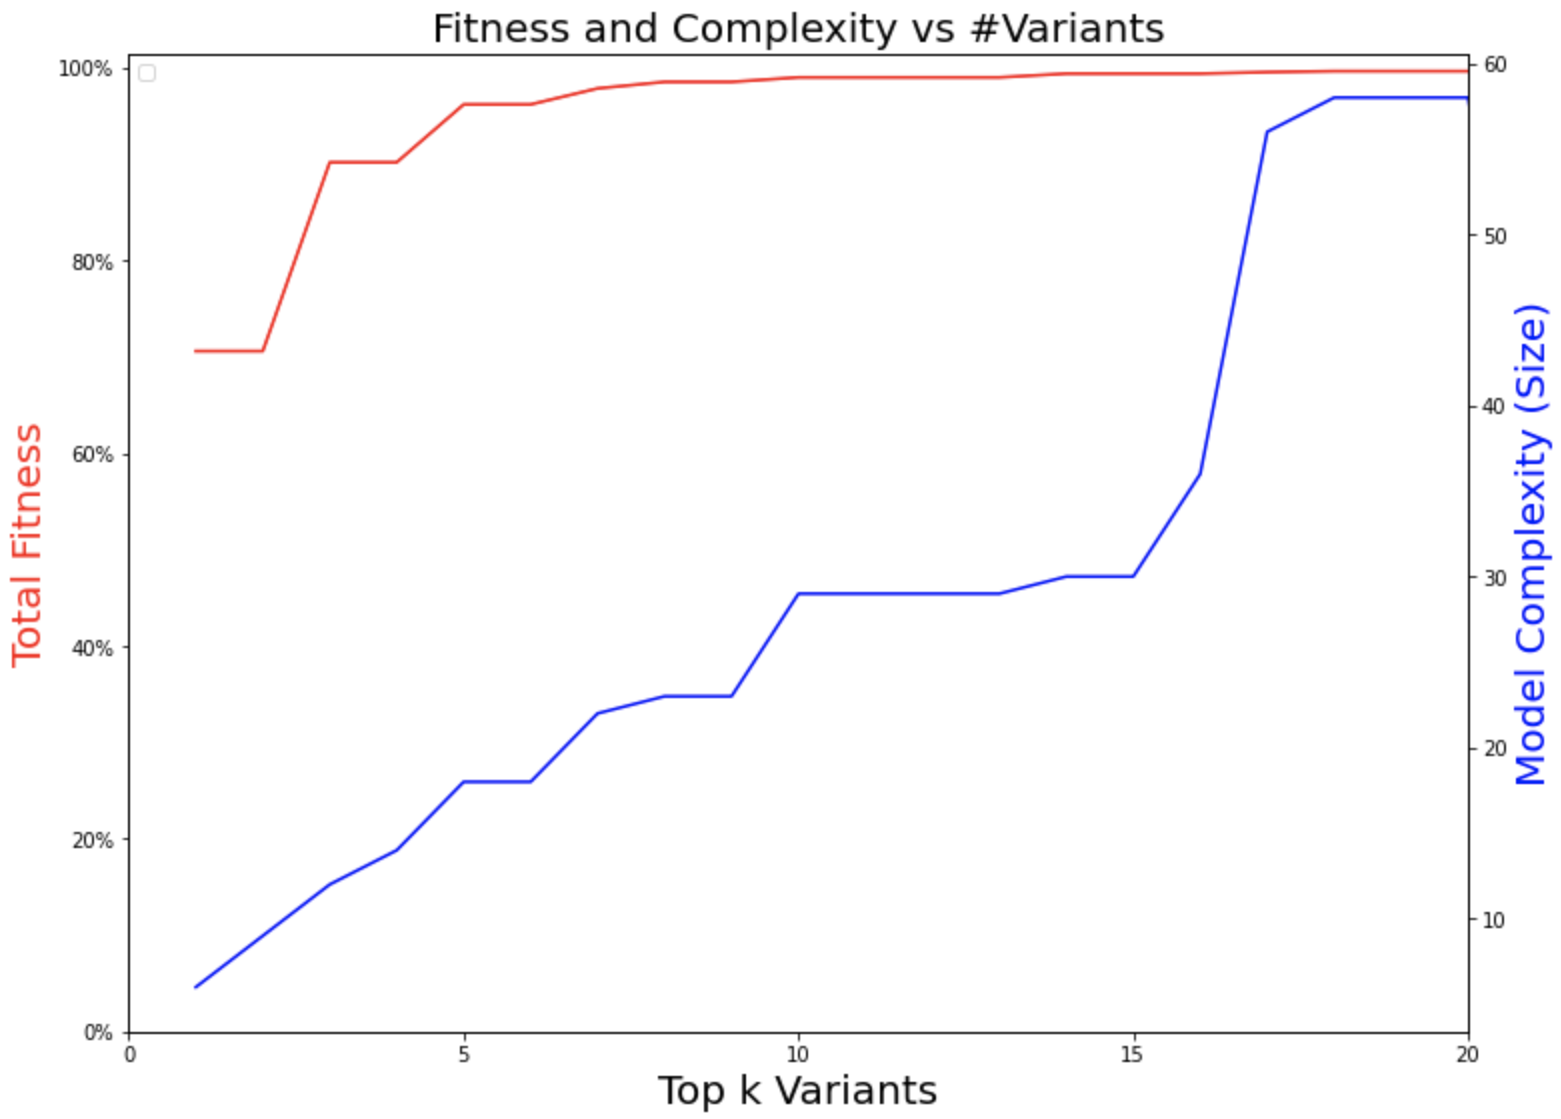
\includegraphics[width=0.40\textwidth]{images/tradeoff.png}}
\caption{Fitness and Complexity vs Top $k$ Variants.}
\label{fig-tradeoff}
\end{figure}

The sweat spots happen at $k = 5$, which can explain 96\% of the traces.
Moreover,
it was able to properly capture the submission, approval, rejection,
resubmission, and the final payment. It represents the best tradeoff
between fitness and model complexity. It would be interesting to further
expand the idea of conformance checking as a way to help build the model,
and we have only just scratched the surface.


%\begin{figure}[htbp]
%\centerline{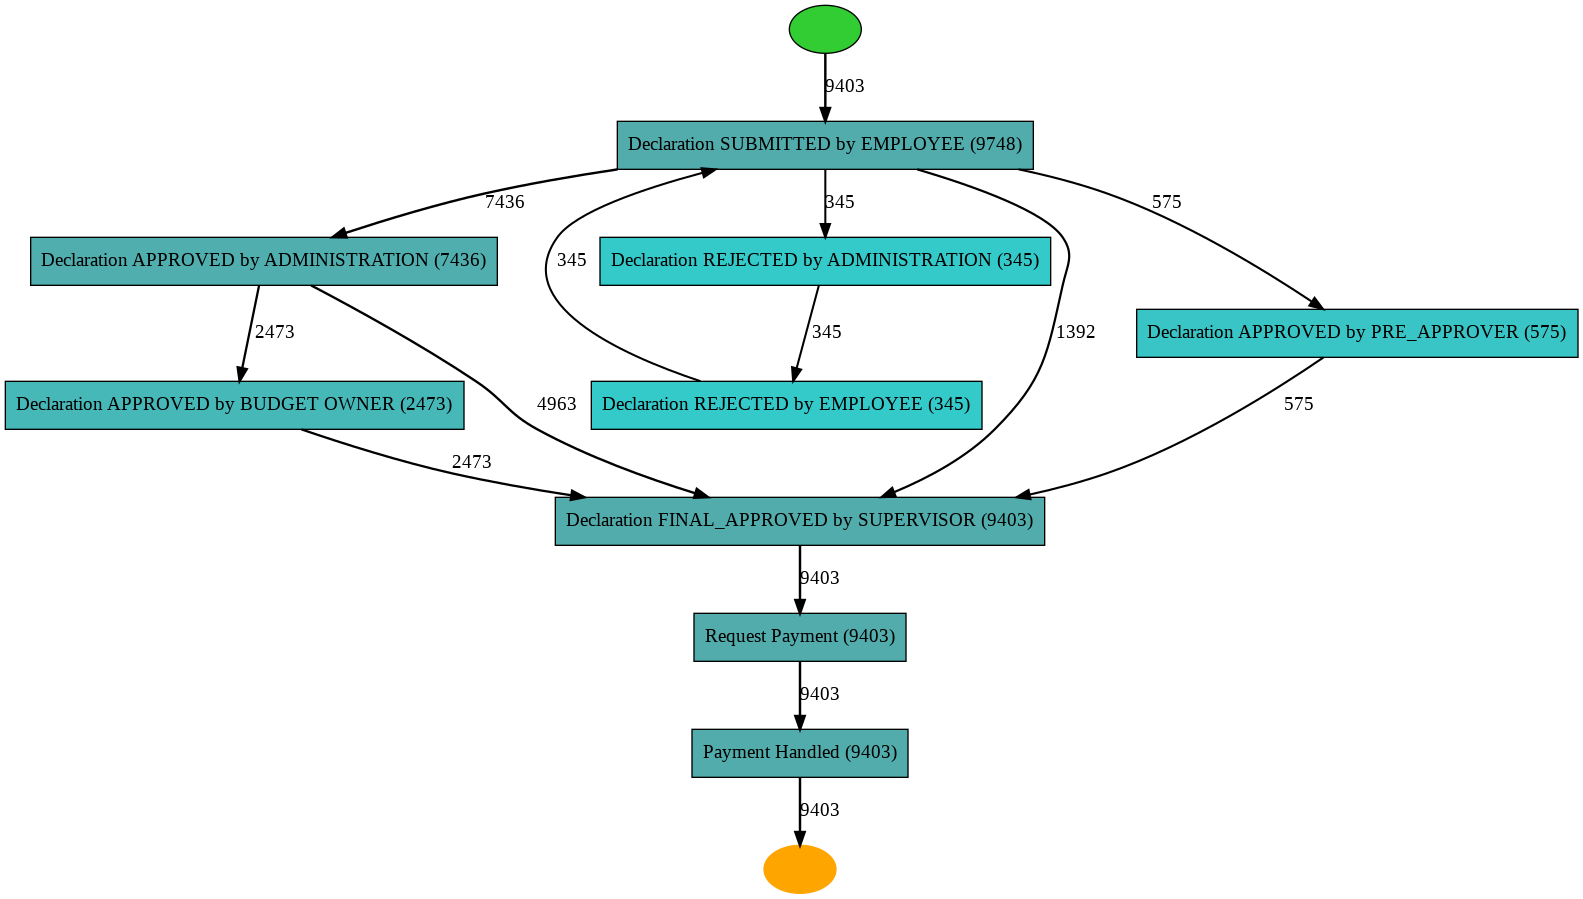
\includegraphics[width=0.45\textwidth]{images/heuristics_net_5.png}}
%\caption{Heuristics Net when using the Top 5 Variants.}
%\label{fig}
%\end{figure}

\subsection{Machine Learning and Timely
Analysis}

Another area of interest is to apply machine learning techniques to
perform (1) flow analysis to predict likelihood of resubmission,
rejection, payment delay, or over-budget based on other variables (time
since submission, request amount, prior owner approval), and (2) timing
analysis to determine the average expected time before the trace completes.
This provides
important clues to administrators and employees alike about the time
frame of payment in the best-case scenario. We are also interested in
detecting non-compliance \textit{as it happens} and sending alerts to
administrators.

\section{Conclusion}
\label{section-conclusion}

In conclusion, we have completed a process mining case study and
demonstrated the effectiveness of modern process mining techniques
in identifying bottlenecks in the travel reimbursement
process. We are encouraged by the power of the \textsc{pm4py} platform
and expect much more research and development to go into process mining,
especially in the direction of process discovery in the era of machine learning.

\bibliographystyle{plain}
\bibliography{paper}{}

% \begin{center}
% \noindent\rule{0.5\columnwidth}{0.4pt}
% \end{center}

\section{Contributions}

We would like to thank Professor Mahima Agumbe Suresh for her teaching,
encouragement, and devotion to helping us and other students succeed.
The following is a breakdown of our individual contributions:

\begin{itemize}
\item \textbf{Martin Alvarez-Lopez} -- advocated for the original proposal,
and set the overall direction of the project. He contributed to
data preparation, the main body of work on process mining, prepared
and gave the main part of the presentation.

\item
\textbf{Carlos Hernandez} -- wrote the first draft of the term paper,
completed with extensive literature survey, project outline,
report template, as well as a significant portion of the writeup.

\item
\textbf{Hardy Leung} -- did an early investigation on \textsc{pm4py}, and
worked on conformance analysis. He also migrated the paper to the IEEE
template, and wrote the second half of the term paper.

\item
\textbf{Divyam Sobti} -- worked closely with Martin A.~on data preparation and
conducted the main investigation on process mining. He set up the CoLab
environment, and contributed to report writing as well.

\end{itemize}

\end{document}
